% !TeX root = ../libro.tex
% !TeX encoding = utf8

\setchapterpreamble[c][0.75\linewidth]{%
	\sffamily
  \emph{La ciencia de la computación no trata sobre ordenadores de la misma manera en que la astronomía no trata sobre telescopios.}
 \begin{flushright} — Edsger W. Dijkstra, \cite{Haines1993}\end{flushright}
% \\[8pt]
	\par\bigskip
}
%\vspace{28pt}

\chapter{El problema de la parada}\label{ch:problema-parada}

En el capítulo anterior, mencionamos que las máquinas de Turing y los programas en Python son equivalentes en términos de los ``problemas'' que pueden resolver. En este capítulo, definiremos formalmente la noción de problema y nos adentraremos en uno de los ejes centrales de la teoría de la computación: la decidibilidad (\cref{sec:problemas-decidibles}).

A continuación, procederemos a introducir la máquina universal (\cref{sec:universalidad}), un concepto que introdujo Turing al presentar su modelo de computación \cite{Turing1937}. Esta máquina nos servirá para encontrar problemas no decidibles (\cref{sec:problemas-no-decidibles}). Finalmente, introduciremos el concepto de reducción (\cref{sec:reducciones}), que nos permitirá encontrar aun más problemas no decidibles.

Haremos todo esto para deducir el resultado principal de este capítulo: la no decidibilidad del problema de la parada (\cref{sec:problema-parada}). Este problema es extremadamente relevante, no solo a nivel histórico, sino será uno de los pilares de la demostración prinicipal de este trabajo, que haremos en el \cref{ch:teorema-incompletitud}.

\section{Problemas decidibles}\label{sec:problemas-decidibles}

Comenzamos, como hemos prometido, definiendo de forma precisa qué es un problema. \cite{MacCormick2018,Sipser2012}

% ====================
\begin{definicion}[Problema computacional]\label{def:problema-computacional}
Un \emph{problema computacional} (o \emph{problema}\index{problema}\index{problema!computacional}) $F$\footnote{Llamamos a los problemas computacionales $F$ y no $P$ para distinguirlos de los programas en Python.} es una función $F:X \longrightarrow Y$, donde:
\begin{itemize}
    \item $X$ es el conjunto de \emph{entradas}. Un elemento $x\in X$ se llama una \emph{entrada}.\index{entrada!de un problema}
    \item $Y$ es el conjunto de \emph{soluciones}. Un elemento $y\in Y$ se llama una \emph{solución}.\index{solución}
\end{itemize}

Dado un $x\in X$ llamamos a $F(x)$ la \emph{solución} de $x$.
\end{definicion}
% ====================

Un problema no es más que una función que mapea entradas a salidas, a las que llamamos soluciones. Cualquier problema puede reducirse a esta terminología, por muy complejo que sea. Veamos la primera descripción de un problema.

% ====================
\begin{problema}
\begin{framed}
$$\text{\textsc{CicloHamiltoniano}}$$

\begin{itemize}
    \item \textbf{Entrada:} un grafo $G$.
    \item \textbf{Solución:} los ciclos hamiltonianos presentes en $G$.
\end{itemize}
\end{framed}
\caption{\textsc{CicloHamiltoniano}}
\label{prob:ciclo-hamiltoniano}
\end{problema}
% ====================

Vamos a definir los conjuntos de entrada y salida del \cref{prob:ciclo-hamiltoniano}.\index{ciclo hamiltoniano} La entrada a nuestro problema es un grafo $G$, que no es más que un conjunto de vértices $V$ y una matriz de adyacencia $A$ representando sus arcos ($G=(V,A)$). Como salida, tendremos un conjunto de $n$ caminos en $G$, $\pi_1,\pi_2,...,\pi_n$ (es posible que un grafo tenga ningún, uno o varios ciclos hamiltonianos). Podemos especificar los caminos como subconjuntos ordenados de $V$.

% ====================
\begin{figure}[H]
\centering
\vspace*{8pt}


\tikzset{every picture/.style={line width=0.75pt}} %set default line width to 0.75pt        

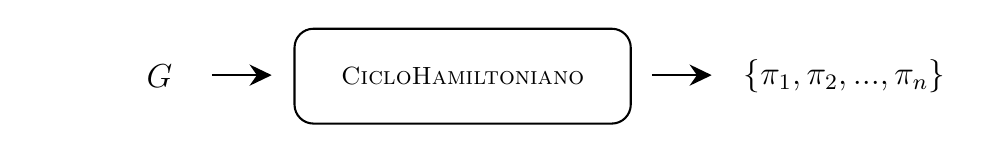
\begin{tikzpicture}[x=0.75pt,y=0.75pt,yscale=-1,xscale=1]
%uncomment if require: \path (0,629); %set diagram left start at 0, and has height of 629

%Rounded Rect [id:dp014958459164192917] 
\draw   (250,537.64) .. controls (250,532.59) and (254.09,528.5) .. (259.14,528.5) -- (402.86,528.5) .. controls (407.91,528.5) and (412,532.59) .. (412,537.64) -- (412,565.06) .. controls (412,570.11) and (407.91,574.2) .. (402.86,574.2) -- (259.14,574.2) .. controls (254.09,574.2) and (250,570.11) .. (250,565.06) -- cycle ;
%Straight Lines [id:da560650477859397] 
\draw    (210.17,550.86) -- (236,550.86) ;
\draw [shift={(239,550.86)}, rotate = 180] [fill={rgb, 255:red, 0; green, 0; blue, 0 }  ][line width=0.08]  [draw opacity=0] (10.72,-5.15) -- (0,0) -- (10.72,5.15) -- (7.12,0) -- cycle    ;
%Straight Lines [id:da283131752424681] 
\draw    (422.17,550.86) -- (448,550.86) ;
\draw [shift={(451,550.86)}, rotate = 180] [fill={rgb, 255:red, 0; green, 0; blue, 0 }  ][line width=0.08]  [draw opacity=0] (10.72,-5.15) -- (0,0) -- (10.72,5.15) -- (7.12,0) -- cycle    ;

% Text Node
\draw (331,551.35) node  [font=\small] [align=left] {\begin{minipage}[lt]{109.82pt}\setlength\topsep{0pt}
\begin{center}
\textsc{CicloHamiltoniano}
\end{center}

\end{minipage}};
% Text Node
\draw (184.98,551.35) node  [font=\large] [align=left] {\begin{minipage}[lt]{88.65pt}\setlength\topsep{0pt}
\begin{center}
$G$
\end{center}

\end{minipage}};
% Text Node
\draw (515,551.35) node  [font=\large] [align=left] {\begin{minipage}[lt]{88.4pt}\setlength\topsep{0pt}
\begin{center}
$\{\pi_1, \pi_2, ..., \pi_n\}$
\end{center}

\end{minipage}};


\end{tikzpicture}

\caption{Esquema de \textsc{CicloHamiltoniano}}
\label{fig:esquema-ciclohamiltoniano}
\end{figure}
% ====================

Para probar los resultados de nuestro trabajo, utilizaremos un subconjunto de problemas: aquellos cuya salida es únicamente \emph{`sí'} o \emph{`no'}. Los llamaremos \emph{problemas de decisión}.

% ====================
\begin{definicion}[Problema de decisión]\label{def:problema-decision}
Dado un alfabeto $A$, un \emph{problema de decisión}\index{problema!de decisión}\footnote{Al referirnos a un ``problema'' sin especificar si es computacional o de decisión, no entraremos en ambigüedad: basta ver las salidas para saber si es de decisión.} es un problema computacional $F:X\longrightarrow Y$ en el que $Y = \{\emph{`sí'}, \emph{`no'}\}$.
\end{definicion}
% ====================

Cualquier problema computacional puede ``transformarse'' en un problema de decisión preguntándonos por la existencia de soluciones. Un ejemplo de esto lo vemos en el \cref{prob:hay-ciclo-hamiltoniano}.

% ====================
\vspace{8pt}
\begin{problema}
\begin{framed}
$$\text{\textsc{HayCicloHamiltoniano}}$$

\begin{itemize}
    \item \textbf{Entrada:} codificación de un grafo $G$.
    \item \textbf{Solución:} si hay al menos un ciclo hamiltoninano en $G$.
\end{itemize}
\end{framed}
\caption{\textsc{HayCicloHamiltoniano}}
\label{prob:hay-ciclo-hamiltoniano}
\end{problema}
% ====================

Este problema es de decisión, pues no pregunta explícitamente por \emph{cuáles} son los ciclos hamiltonianos presentes en un determinado grado, sino por si \emph{existe} un ciclo hamiltoniano en él. Evidentemente, este tipos de problemas son más restrictivos que los problemas computacionales generales, pero tienen mucho más interés a la hora de hablar de decidibilidad, como veremos más adelante.

% ====================
\begin{figure}[H]
\centering
\vspace*{8pt}


\tikzset{every picture/.style={line width=0.75pt}} %set default line width to 0.75pt        

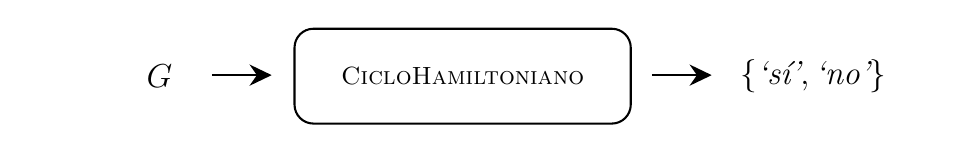
\begin{tikzpicture}[x=0.75pt,y=0.75pt,yscale=-1,xscale=1]
%uncomment if require: \path (0,629); %set diagram left start at 0, and has height of 629

%Rounded Rect [id:dp014958459164192917] 
\draw   (250,537.64) .. controls (250,532.59) and (254.09,528.5) .. (259.14,528.5) -- (402.86,528.5) .. controls (407.91,528.5) and (412,532.59) .. (412,537.64) -- (412,565.06) .. controls (412,570.11) and (407.91,574.2) .. (402.86,574.2) -- (259.14,574.2) .. controls (254.09,574.2) and (250,570.11) .. (250,565.06) -- cycle ;
%Straight Lines [id:da560650477859397] 
\draw    (210.17,550.86) -- (236,550.86) ;
\draw [shift={(239,550.86)}, rotate = 180] [fill={rgb, 255:red, 0; green, 0; blue, 0 }  ][line width=0.08]  [draw opacity=0] (10.72,-5.15) -- (0,0) -- (10.72,5.15) -- (7.12,0) -- cycle    ;
%Straight Lines [id:da283131752424681] 
\draw    (422.17,550.86) -- (448,550.86) ;
\draw [shift={(451,550.86)}, rotate = 180] [fill={rgb, 255:red, 0; green, 0; blue, 0 }  ][line width=0.08]  [draw opacity=0] (10.72,-5.15) -- (0,0) -- (10.72,5.15) -- (7.12,0) -- cycle    ;

% Text Node
\draw (331,551.35) node  [font=\small] [align=left] {\begin{minipage}[lt]{109.82pt}\setlength\topsep{0pt}
\begin{center}
\textsc{CicloHamiltoniano}
\end{center}

\end{minipage}};
% Text Node
\draw (184.98,551.35) node  [font=\large] [align=left] {\begin{minipage}[lt]{88.65pt}\setlength\topsep{0pt}
\begin{center}
$G$
\end{center}

\end{minipage}};
% Text Node
\draw (500,551.35) node  [font=\large] [align=left] {\begin{minipage}[lt]{88.4pt}\setlength\topsep{0pt}
\begin{center}
$\{\text{\emph{`sí'}}, \text{\emph{`no'}}\}$
\end{center}

\end{minipage}};


\end{tikzpicture}

\caption{Esquema de \textsc{HayCicloHamiltoniano}}
\label{fig:esquema-hayciclohamiltoniano}
\end{figure}
% ====================
En el caso de los problemas de decisión, tiene sentido hablar de su complementario.

% ====================
\begin{definicion}[Problema complementario]\label{def:problema-complementario}
Dado un problema de decisión $D$, definimos su \emph{problema complementario}\index{problema!complementario}\index{problema!contrario} (o \emph{problema contrario}), denotado $\overline{D}$, como:
$$
    \overline{D}(a) = \text{\emph{`sí'}} \iff D(a) = \text{\emph{`no'}},\;\;\;\;\;\overline{D}(a) = \text{\emph{`no'}} \iff D(a) = \text{\emph{`sí'}}
$$
\end{definicion}
% ====================

En algunas ocasiones, usaremos la notación C- para referirnos al problema complementario: dado un problema \textsc{Problema}, llamaremos \textsc{C-Problema} a su problema contrario.

\vspace{8pt}

Para continuar, es necesario comentar algunas particularidades de los programas en Python para tratar con problemas. Como bien sabemos, los programas sólo aceptan \emph{strings} como entrada y \emph{strings} como solución. Podemos pensar en un programa en Python $P$ como en una función
$$
    P : S \longrightarrow S
$$
donde $S$ es el conjunto de todos los \emph{strings} posibles en Python. Dependiendo de la versión de Python, este conjunto será mayor o menor.\footnote{En las últimas versiones de Python, es posible trabajar con UTF-8.}

Para que un ordenador pueda resolver un problema, necesitaremos codificar las entradas y las soluciones del problema mediante un formato que pueda entender: las cadenas de caracteres (\emph{strings}). Tal y como se demuestra en la \cref{prop:f-s}, para cualquier problema podremos suponer que las entradas y soluciones están codificadas\index{codificación} mediante \emph{strings}.\index{codificación!de entradas y soluciones}

Esto no supone una restricción: las entradas y las soluciones pueden ser codificadas como cadenas de caracteres. Deberemos, sin embargo, tener en cuenta que es posible que haya entradas que no sean una codificación correcta de una entrada del problema original. En tal caso, asignaremos la salida \palabra{no} a tal entrada.

Vemos un ejemplo de esto en el \cref{prob:ciclo-hamiltoniano-codificacion}. Este problema tendrá asociada una cierta codificación para las entradas y las soluciones. Observa que este problema es idéntico al \cref{prob:ciclo-hamiltoniano}, y que podemos traducir las entradas y las soluciones de uno y otro conociendo la codificación elegida.

% ====================
\begin{problema}
\begin{framed}
$$\text{\textsc{CicloHamiltonianoCodificación}}$$

\begin{itemize}
    \item \textbf{Entrada:} codificación de un grafo $G$.
    \item \textbf{Solución:} codificación de los ciclos hamiltonianos presentes en $G$.
\end{itemize}
\end{framed}
\caption{\textsc{CicloHamiltonianoCodificación}}
\label{prob:ciclo-hamiltoniano-codificacion}
\end{problema}
% ====================

En el caso de los problemas de decisión, las soluciones siempre serán \palabra{sí} y \palabra{no}. Nótese que \palabra{no} será solución tanto para las instancias negativas del problema como para las codificaciones incorrectas.

De aquí en adelante, todos los problemas tendrán cadenas de caracteres como entradas y soluciones.

A continuación, concretaremos la relación entre programas y problemas que ya veníamos intuyendo desde el \cref{ch:programas-python-maquinas-turing}.

\begin{definicion}[Resolver y decidir]\label{def:resolver-decidir}
Dado un problema $F:S\longrightarrow S$ y un programa $P$, diremos que $P$ \emph{resuelve}\index{resolver} $F$ si, para cada entrada $I\in S$, $P$ para y devuelve un \emph{string} tal que $P(I)=F(I)$.

Si $F$ es un problema de decisión resuelto por $P$, diremos que $P$ \emph{decide}\index{decidir} $F$.
\end{definicion}

Un problema computacional describe lo que queremos resolver. Un programa describe la forma particular de computar la solución a un problema.

Es muy importante destacar que, en la definición anterior, es necesario que $P$ \emph{pare} para todas las entradas. O, lo que es lo mismo, si $P$ cicla para alguna entrada, no resuelve $F$. Esta condición puede relajarse dando lugar a problemas \emph{semidecidibles} (véase la \cref{sec:problemas-semidecidibles}).

Esta característica de ``resolver'' es realmente una propiedad del problema, y no del programa. En el caso de los problemas de decisión, esto nos conduce a la definición de \emph{computabilidad}.

\begin{definicion}[Problema computable y problema decidible]\label{def:decidible}
Sea $F$ un problema computacional. Si existe un programa $P$ que lo resuelve, decimos que el problema es \emph{computable}.\index{problema!computable}

En el caso en el que $D$ sea un problema de decisión, si existe un programa $P$ que lo decida decimos que el problema es \emph{decidible}.\index{problema!decidible}
\end{definicion}

Veamos un problema más sencillo que el \cref{prob:ciclo-hamiltoniano}. El \cref{prob:mas-a-que-b}, \textsc{MásAQueB}, tiene como entrada una palabra del alfabeto $\{\palabra{a}, \palabra{b}\}$, y como solución \palabra{sí} en caso de que la palabra tenga más \palabra{a} que \palabra{b}, y \palabra{no} en caso contrario o en el caso de que la codificación sea incorrecta. Para este problema, la codificación es incorrecta si la entrada es una cadena de caracteres que no conforma una palabra del alfabeto $\{\palabra{a}, \palabra{b}\}$.

Evidentemente, \textsc{MásAQueB} es un problema de decisión. Ahora nos queda preguntarnos si este problema es decidible. La respuesta es afirmativa, y se demuestra en detalle en la \cref{prop:masaqueb-decidible}.

% ====================
\begin{problema}
\begin{framed}
$$\text{\textsc{MásAQueB}}$$

\begin{itemize}
    \item \textbf{Entrada:} una cadena de caracteres del alfabeto $\{\palabra{a}, \palabra{b}\}$.
    \item \textbf{Salida:} si la cadena de caracteres tiene más \palabra{a} que \palabra{b}.
\end{itemize}
\end{framed}
\caption{\textsc{MásAQueB}}
\label{prob:mas-a-que-b}
\end{problema}
% ====================

Si queremos saber si el problema es decidible, deberemos escribir un programa que lo resuelva y nunca cicle, y que tenga en cuenta las codificaciones incorrectas. Esto es precisamente lo que hace el programa a continuación:

\vspace{8pt}

% ====================
\begin{lstlisting}[language=Python, caption=\lstinline{mas_a_que_b.py},label={lst:mas-a-que-b}]
import utilidades|\label{line:mas-a-que-b-import}|

def mas_a_que_b(palabra):|\label{line:mas-a-que-b-main}|
    # comprobamos si la codificación es correcta, es decir (si es del alfabeto {'a', 'b'}), si no es correcta devolvemos 'no'
    if not utilidades.en_alfabeto(palabra, {'a', 'b'}):|\label{line:mas-a-que-b-alfabeto}|
        return 'no'

    if palabra.count('a') > palabra.count('b'):|\label{line:mas-a-que-b-contar}|
        return 'sí'|\label{line:mas-a-que-b-si}|

    return 'no'|\label{line:mas-a-que-b-no}|
\end{lstlisting}
% ====================

Explicamos el programa brevemente. Vemos en la \cref{line:mas-a-que-b-main} la función \emph{main} del programa, que acepta una palabra como entrada. En la \cref{line:mas-a-que-b-alfabeto} comprobamos que la palabra pertenezca al alfabeto $\{\palabra{a}, \palabra{b}\}$ mediante la función \texttt{en\_alfabeto} de la librería \texttt{utilidades} (que importamos en la \cref{line:mas-a-que-b-import}). En caso de que la palabra no pertenezca al alfabeto, devolvemos \palabra{no}, pues la codificación es incorrecta. Si pertenece al alfabeto, llegamos a la \cref{line:mas-a-que-b-contar} y comprobamos si tiene más \palabra{a} que \palabra{b}. En caso de ser así, devuelve \palabra{sí} en la \cref{line:mas-a-que-b-si} y, si no, devuelve \palabra{no} en la \cref{line:mas-a-que-b-no}. Vemos algunas de las salidas del programa \texttt{mas\_a\_que\_b.py} en la \cref{tab:masaqueb-io}.

% ====================
\begin{tabla}
\begin{table}[H]
\centering
\begin{tabular}{@{}lc@{}}
\toprule
Comando  & Salida \\ \midrule
\texttt{mas\_a\_que\_b(\palabra{abaab})} & \palabra{sí} \\
\texttt{mas\_a\_que\_b(\palabra{abbab})} & \palabra{no} \\
\texttt{mas\_a\_que\_b(\palabra{})} & \palabra{no} \\
\texttt{mas\_a\_que\_b(\palabra{abaabc})} & \palabra{no} \\ \bottomrule
\end{tabular}
\end{table}
\vspace{-8pt}
\caption{Ejemplos de salidas de \texttt{mas\_a\_que\_b.py}}
\label{tab:masaqueb-io}
\end{tabla}
% ====================

Dado que hemos encontrado un programa \texttt{mas\_a\_que\_b.py} que decide \textsc{MásAQueB}, el problema \textsc{MásAQueB} es decidible.

\begin{proposicion}\label{prop:masaqueb-decidible}
El problema \textsc{MásAQueB} es decidible.
\end{proposicion}
\begin{proof}
El \cref{lst:mas-a-que-b} decide \textsc{MásAQueB}. En efecto, vemos que el programa para para todas las entradas $I\in S$ y devuelve:
\begin{itemize}
    \item Si $I \notin \{\palabra{a}, \palabra{b}\}$, es $P(I)=\textsc{MásAQueB}(I)=\palabra{no}$ (entrada con codificación incorrecta).
    \item Si $I \in \{\palabra{a}, \palabra{b}\}$:
    \begin{itemize}
        \item Si $I$ tiene más \palabra{a} que \palabra{b}, es $P(I)=\textsc{MásAQueB}(I)=\palabra{sí}$.
        \item Si $I$ no tiene más \palabra{a} que \palabra{b}, es $P(I)=\textsc{MásAQueB}(I)=\palabra{no}$.
    \end{itemize}
\end{itemize}
\end{proof}

Una nota respecto a nuestra definición de decidibilidad. Normalmente, en los cursos de teoría de la computación, esta definición se hace respecto a máquinas de Turing. Sin embargo, al haber probado la equivalencia con los programas en Python en el \cref{ch:programas-python-maquinas-turing}, podemos definirlo directamente en términos de programas. Según la definición de máquinas de Turing, sin embargo, también podríamos probar que \textsc{MásAQueB} es decidible: basta ver que la máquina $M_{\#a>\#b}$ del \cref{ej:mt-1} decide el problema, pues nunca para y acepta las palabras que tienen más $a$ que $b$.

\section{Universalidad}\label{sec:universalidad}

En la \cref{sec:equivalencia} vimos cómo podemos simular una máquina de Turing mediante un programa en Python. Pero, ¿es posible simular un programa en Python mediante un programa en Python? La respuesta es sí, y no debería resultar sorprendente, pues muchas de las operaciones que ejecutamos en el día a día en nuestros ordenadores involucran este tipo de simulaciones.

Por ejemplo, al ejecutar un programa en Python cualquiera, estamos ejecutando el intérprete de Python, que es un programa en sí mismo.

Esta idea de ``programas que ejecutan programas'' puede parecer obvia, pero realmente fue revolucionaria en su tiempo, y es el motivo por el que los ordenadores personales son hoy la norma, llegando a encontrarse hasta en nuestros bolsillos. Quizás la cosa más increíble que puede hacer un ordenador es ejecutar \emph{cualquier cosa} -- no simplemente un conjunto de programas fijos preinstalados por el fabricante.

Para entender cómo esto puede ser posible en el caso de un programa en Python, deberemos de entender el funcionamiento de la función nativa \texttt{exec} \cite{Lutz2013}. Si probamos en el intérprete:
\begin{lstlisting}[numbers=none,frame=none]
>>> exec("print('resultado:', 11+2)")
resultado: 13
\end{lstlisting}
Vemos cómo a \texttt{exec} pasamos una sentencia en Python en forma de \emph{string}, y la ejecuta. De hecho, observa cómo ha ejecutado la suma $11+2$, y no simplemente ha imprimido \palabra{11+2}.

Esto podemos llevarlo un paso más allá: dentro de \texttt{exec} podemos insertar varias líneas e incluso definir funciones, variables, etc.
\begin{lstlisting}[numbers=none,frame=none]
>>> exec("def hola(nombre):\n\tprint(f'Hola, {nombre}')\nhola('TFG')")
Hola, TFG
\end{lstlisting}
\vspace{-8pt}
Una vez conocemos esto, podemos crear el siguiente programa:\index{máquina universal}
\vspace{8pt}
% ====================
\begin{lstlisting}[language=Python, caption=\lstinline{maquina_universal.py},label={lst:maquina-universal}]
import utilidades

def maquina_universal(programa, entrada):|\label{line:maquina-universal-main}|
    # esto define las funciones del programa, pero no las ejecuta
    try:|\label{line:maquina-universal-try}|
        exec(programa)|\label{line:universal-exec}|
    except Exception as excepcion:|\label{line:maquina-universal-except}|
        return 'error: ' + str(excepcion)|\label{line:maquina-universal-except-return}|

    # extraemos una referencia a la función main, que está definida localmente
    main = utilidades.extraer_main(programa, locals())|\label{line:maquina-universal-main-ref}|

    # invocamos la función
    return main(entrada)|\label{line:maquina-universal-return}|
\end{lstlisting}
% ====================

Veamos qué es lo que hace el \cref{lst:maquina-universal}. En primer lugar, vemos en la \cref{line:maquina-universal-main} que la función \emph{main} admite dos parámetros: un programa y una entrada, ambos \emph{string}. En la \cref{line:universal-exec} ejecutamos el programa definido en \texttt{programa}, tal y como explicamos anteriormente. Esta línea está dentro de un bloque \texttt{try-except} dado que es posible que el programa esté mal definido, en cuyo caso se lanza una excepción. Esta excepción la cazamos, dado que según la \cref{def:programa-siso}, el programa no debe lanzar ninguna excepción. En la \cref{line:maquina-universal-except} vemos que, de haber una excepción, entraremos a la \cref{line:maquina-universal-except-return}, que devuelve un \emph{string} con los detalles del error.

Si no hay error, la \cref{line:universal-exec} se ejecutará satisfactoriamente, y las funciones que se definan en \texttt{programa} serán accesibles desde la función \texttt{universal} (\cref{line:maquina-universal-main}). En concreto, todas las definiciones de \texttt{programa} serán accesibles desde \texttt{locals()}. Aprovechamos esto en la \cref{line:maquina-universal-main-ref}, donde extraemos una referencia a la función \emph{main} de \texttt{programa}, que finalmente ejecutamos con la entrada \texttt{entrada} en la \cref{line:maquina-universal-return}.

Hemos logrado crear un programa en Python que es capaz de ejecutar otro programa. Esto nos permitirá ejecutar cualquiera de los problemas que hemos creado, sin más que pasar el programa a un \emph{string}. En la librería \texttt{utilidades} se encuentra la función \texttt{leer}, que dada una ruta a un archivo devuelve el archivo en \emph{string}.

Algunos ejemplos de ejecución de \texttt{maquina\_universal.py} se especifican en la tabla siguiente.

% ====================
\begin{tabla}
\begin{table}[H]
\centering
\begin{tabular}{@{}lc@{}}
\toprule
Comando  & Salida \\ \midrule
\texttt{maquina\_universal(\palabra{no es un programa}, \palabra{una entrada cualquiera})} & \texttt{\textquotesingle}\texttt{error}$...$\texttt{\textquotesingle} \\
\texttt{maquina\_universal(leer(\palabra{./mas\_a\_que\_b.py}), \palabra{abaab})} & \palabra{sí} \\
\texttt{maquina\_universal(leer(\palabra{./mas\_a\_que\_b.py}), leer(\palabra{./mas\_a\_que\_b.py}))} & \palabra{no} \\
\texttt{maquina\_universal(leer(\palabra{./mas\_a\_que\_b\_v2.py}), leer(\palabra{./mas\_a\_que\_b.py}))} & \palabra{sí} \\
\texttt{maquina\_universal(leer(\palabra{./si.py}), leer(\palabra{./mas\_a\_que\_b.py}))} & \palabra{sí} \\
\texttt{maquina\_universal(leer(\palabra{./simula\_turing.py}),} & \palabra{sí}\\
\hspace{16pt}\texttt{utilidades.MAU(leer(\palabra{./maquinas\_turing/mas\_a\_que\_b.mt}), \palabra{abaab}))} &  \\ \bottomrule
\end{tabular}
\end{table}
\vspace{-8pt}
\caption{Ejemplos de salidas de \texttt{maquina\_universal.py}}
\label{tab:maquina-universal-io}
\end{tabla}
% ====================
En la primera fila, podemos ver que, al insertar un programa inválido como entrada, la salida de \texttt{maquina\_universal.py} será de error. En la segunda fila, ejecutamos el programa \texttt{mas\_a\_que\_b.py} con la entrada \palabra{aaba}. El resultado es exactamente el esperado (observa la primera fila de la \cref{tab:masaqueb-io}).

En la tercera fila, usamos el propio código de \texttt{mas\_a\_que\_b.py} como entrada para sí mismo. Esto tiene sentido, dado que un programa, como hemos comentado, no es más que un \emph{string}. Recuerda que el \cref{lst:mas-a-que-b} trata entradas fuera del alfabeto $\{\palabra{a}, \palabra{b}\}$ como una entrada incorrecta, y es por ello por lo que la salida es \palabra{no}. Modificamos esto en el \cref{lst:mas-a-que-b-v2}, en el que acpetamos cualquier entrada y contamos su número de \palabra{a} y \palabra{b}. Vemos cómo, en la cuarta fila, la salida es \palabra{sí}, dado que en este caso la codificación es correcta.

\vspace{8pt}
% ====================
\begin{lstlisting}[language=Python, caption=\lstinline{mas_a_que_b_v2.py},label={lst:mas-a-que-b-v2}]
def mas_a_que_b_v2(palabra):
    if palabra.count('a') > palabra.count('b'):
        return 'sí'

    return 'no'
\end{lstlisting}
% ====================

En la quinta fila, utilizamos el \cref{lst:si}. Este programa siempre devuelve \palabra{sí}, independientemente de la entrada que pasemos. Evidentemente, este programa es el que decide el \cref{prob:si} (es decir, \textsc{Sí} es decidible).\label{lab:si-decidible}
\vspace{8pt}
% ====================
\begin{lstlisting}[language=Python, caption=\lstinline{si.py},label={lst:si}]
def si(entrada):
    # siempre devuelve 'sí'
    return 'sí'
\end{lstlisting}
% ====================
% ====================
\begin{problema}
\begin{framed}
$$\text{\textsc{Sí}}$$

\begin{itemize}
    \item \textbf{Entrada:} una cadena de caracteres cualquiera.
    \item \textbf{Salida:} \palabra{sí}.
\end{itemize}
\end{framed}
\caption{\textsc{Sí}}
\label{prob:si}
\end{problema}
% ====================
En la sexta y última fila vemos cómo \texttt{maquina\_universal.py} puede ejecutar cualquier programa en Python, incluso el \cref{lst:simula-turing}, que simula máquinas de Turing. Como entrada al programa pasamos la codificación de una máquina de Turing y la entrada. En efecto, la salida sigue siendo \palabra{sí}.

Esta capacidad de los programas de ejecutarse a sí mismos es extremadamente interesante y es una característica que nos causará muchos problemas, como veremos en la \cref{sec:problemas-no-decidibles}.
%Lo que hemos hecho, realmente es resolver el problema \textsc{Universal}. Es fácil comprobar que el \cref{lst:universal} resuelve el \cref{prob:universal}. WIP NO DECIDE
\vspace{8pt}

% ====================
%\begin{problema}
%\begin{framed}
%$$\text{\textsc{Universal}}$$
%
%\begin{itemize}
%    \item \textbf{Entrada:} un programa $P$ y una entrada $I$.
%    \item \textbf{Salida:} $P(I)$, el resultado de ejecutar $P$ con entrada $I$.
%\end{itemize}
%\end{framed}
%\caption{\textsc{Universal}}
%\label{prob:universal}
%\end{problema}
% ====================

Llamamos a una máquina \emph{universal}\index{máquina universal} si es capaz de simular una máquina de Turing, dado que este concepto lo introdujo Turing en su famosa publicación \cite{Turing1937}. Por el resultado de equivalencia (\cref{teo:equivalencia}), vemos que \cref{lst:maquina-universal} es, en efecto, una máquina universal (algo que podíamos intuir con el nombre del programa).

Como vimos al principio, el concepto de universalidad es una constante en los ordenadores que usamos: el hardware es universal, porque puede ser usado para ejecutar cualquier máquina de Turing, del mismo modo que lo es un sistema operativo, pues puede compilar programas que simulan máquinas de Turing. El intérprete de Python también es universal por este mismo motivo, así como la máquina virtual de Java. Incluso un programa en sí mismo (\cref{lst:maquina-universal}) puede ser universal.

\section{Problemas no decidibles}\label{sec:problemas-no-decidibles}

En la \cref{sec:problemas-decidibles} mostramos cómo probar que un problema es decidible, lo cual es sencillo: basta encontrar un programa que lo decida. Sin embargo, probar que un problema no lo es es mucho más complicado. En este apartado encontraremos varios problemas no decidibles.
\vspace{8pt}
% ====================
\begin{problema}
\begin{framed}
$$\text{\textsc{Universal}}$$

\begin{itemize}
    \item \textbf{Entrada:} un programa $P$ y una entrada $I$.
    \item \textbf{Salida:} \palabra{sí} si $P$ está bien definido y $P(I)=\text{\palabra{sí}}$, \palabra{no} en caso contrario.
\end{itemize}
\end{framed}
\caption{\textsc{Universal}}
\label{prob:universal}
\end{problema}
% ====================
Comencemos por el problema \textsc{Universal}.\footnote{Este problema no tiene, inicialmente, relación alguna con la máquina universal que definimos en el \cref{lst:maquina-universal}.} Claramente, se trata de un problema de decisión, pues devuelve \palabra{sí} o \palabra{no}. En esta sección, probaremos que escribir un programa que decida \textsc{Universal} es imposible. En caso de que fuese posible hacerlo, vemos en la \cref{tab:universal-io} las posibles salidas que tendría.
% ====================
\begin{tabla}
\begin{table}[H]
\centering
\begin{tabular}{@{}lc@{}}
\toprule
Comando  & Salida \\ \midrule
\texttt{universal(\palabra{no es un programa}, \palabra{una entrada cualquiera})} & \palabra{no} \\
\texttt{universal(leer(\palabra{./mas\_a\_que\_b\_v2.py}), \palabra{aaba})} & \palabra{sí} \\
\texttt{universal(leer(\palabra{./mas\_a\_que\_b\_v2.py}), leer(\palabra{./mas\_a\_que\_b\_v2.py})} & \palabra{sí} \\
\texttt{universal(leer(\palabra{./si.py}), \palabra{aaba})} & \palabra{sí} \\
\texttt{universal(leer(\palabra{./si.py}), leer(\palabra{./si.py}))} & \palabra{sí} \\ \bottomrule
\end{tabular}
\end{table}
\vspace{-8pt}
\caption{Ejemplos de salidas de \texttt{universal.py}}
\label{tab:universal-io}
\end{tabla}
% ====================
En la primera fila vemos cómo, para codificaciones incorrectas, el programa devuelve \palabra{no}. Las filas siguientes son evidentes, y similares a las de la \cref{tab:maquina-universal-io}.

Introduciremos dos problemas más. El primero de ellos, \textsc{Diagonal}, podemos obtenerlo a partir de \textsc{Universal} (\cref{prob:universal}) con $I=P$.\label{lab:diagonal-a-universal}
\vspace{8pt}
% ====================
\begin{problema}
\begin{framed}
$$\text{\textsc{Diagonal}}$$

\begin{itemize}
    \item \textbf{Entrada:} un programa $P$.
    \item \textbf{Salida:} \palabra{sí} si $P(P)$ está bien definido y $P(I)=\text{\palabra{sí}}$, \palabra{no} en caso contrario.
\end{itemize}
\end{framed}
\caption{\textsc{Diagonal}}
\label{prob:diagonal}
\end{problema}
% ====================
 En caso de existir un programa que decida este problema, vemos en la tabla siguiente las posibles salidas que tendría.
% ====================
\begin{tabla}
\begin{table}[H]
\centering
\begin{tabular}{@{}lc@{}}
\toprule
Comando  & Salida \\ \midrule
\texttt{diagonal(\palabra{no es un programa})} & \palabra{no} \\
\texttt{diagonal(\texttt{leer}(\palabra{./mas\_a\_que\_b\_v2.py}))} & \palabra{sí} \\
\texttt{diagonal(\texttt{leer}(\palabra{./si.py}))} & \palabra{sí} \\
\texttt{diagonal(\texttt{leer}(\palabra{./diagonal.py}))} & \textbf{¿}\palabra{sí} o \palabra{no}\textbf{?}\\ \bottomrule
\end{tabular}
\end{table}
\vspace{-8pt}
\caption{Ejemplos de salidas de \texttt{diagonal.py}}
\label{tab:diagonal-io}
\end{tabla}
% ====================
Las tres primeras salidas no requiren más explicación. Sin embargo, centrémonos en la última: ¿cuál sería el resultado de ejecutar \texttt{diagonal.py} con el código de \texttt{diagonal.py}?

Parece ser que tanto \palabra{sí} como \palabra{no} son ambas respuestas correctas -- basta ver la definición del \cref{prob:diagonal}. Tomando $I$ como \texttt{diagonal.py} y $P$ como el mismo programa, entonces, si $P(I)=\palabra{sí}$, el programa devolverá \palabra{sí}, mentras que si $P(I)=\palabra{no}$, entonces el programa devolverá \palabra{no}.

Llegado a este punto deberíamos sospechar que las cosas no van a ir bien. Terminemos este ``circo recursivo'' con un último problema, \textsc{C-Diagonal}.\footnote{Notar que $\textsc{C-Diagonal}=\overline{\textsc{Diagonal}}$} En caso de existir un programa que lo decida, \texttt{c\_diagonal.py}, vemos sus posibles salidas en la \cref{tab:c-diagonal-io}.
\vspace{8pt}
% ====================
\begin{problema}
\begin{framed}
$$\text{\textsc{C-Diagonal}}$$

\begin{itemize}
    \item \textbf{Entrada:} un programa $P$.
    \item \textbf{Salida:} \palabra{no} si $P(P)$ está bien definido y $P(I)=\text{\palabra{sí}}$, \palabra{sí} en caso contrario.
\end{itemize}
\end{framed}
\caption{\textsc{C-Diagonal}}
\label{prob:c-diagonal}
\end{problema}
% ====================
\vspace{-8pt}
% ====================
\begin{tabla}
\begin{table}[H]
\centering
\begin{tabular}{@{}lc@{}}
\toprule
Comando  & Salida \\ \midrule
\texttt{c\_diagonal(\palabra{no es un programa})} & \palabra{sí} \\
\texttt{c\_diagonal(\texttt{leer}(\palabra{./mas\_a\_que\_b\_v2.py}))} & \palabra{no} \\
\texttt{c\_diagonal(\texttt{leer}(\palabra{./si.py}))} & \palabra{no} \\
\texttt{c\_diagonal(\texttt{leer}(\palabra{./c\_diagonal.py}))} & \textbf{¿}\palabra{sí} o \palabra{no}\textbf{?}\\ \bottomrule
\end{tabular}
\end{table}
\vspace{-8pt}
\caption{Ejemplos de salidas de \texttt{c\_diagonal.py}}
\label{tab:c-diagonal-io}
\end{tabla}
% ====================
Volvemos a repetir la misma pregunta que nos hicimos para el caso de \textsc{Diagonal} (\cref{prob:diagonal}). ¿Qué salida tendría un hipotético programa que lo resolviese, si se usa a sí mismo como entrada? En este caso, esta pregunta es justamente la que nos demuestra que escribir tal programa es imposible. Esto nos indica que el problema \textsc{C-Diagonal} no es decidible. Veamos una demostración más precisa de este hecho.

\begin{proposicion}\label{prop:c-diagonal-no-decidible}
El problema \textsc{C-Diagonal} es no decidible.
\end{proposicion}
\begin{proof}
Supongamos que \textsc{C-Diagonal} es decidible. Entonces, existe un programa en Python \texttt{c\_diagonal.py} que resuelve \textsc{C-Diagonal}. Entonces, podemos preguntarnos por la salida del comando:
\begin{adjustwidth}{30pt}{}
    \texttt{c\_diagonal(\texttt{leer}(\palabra{./c\_diagonal.py}))}
\end{adjustwidth}
Este comando pregunta:
\begin{adjustwidth}{30pt}{}
    ¿Es cierto que \texttt{c\_diagonal.py} \emph{no} devuelve \palabra{sí} cuando se ejecuta a sí mismo?
\end{adjustwidth}
La respuesta a la pregunta anterior puede ser afirmativa o negativa. Veremos que ninguna de ambas puede ser posible.

Si la respuesta es afirmativa, entonces sabemos que \texttt{c\_diagonal.py} no devuelve \palabra{sí} cuando se ejecuta a sí mismo, luego la respuesta debería haber sido negativa -- una contradicción, es decir, la respuesta no puede ser afirmativa.

En caso de que sea la respuesta negativa, entonces \texttt{c\_diagonal.py} devuelve \palabra{no} cuando se ejecuta a sí mismo, luego la respuesta debería haber sido afirmativa -- de nuevo una contradicción, en otras palabras, la respuesta tampoco puede ser negativa.

Concluimos, por tanto, que es imposible escribir el programa \texttt{c\_diagonal.py}. Como no podemos escribir un programa que decida \textsc{C-Diagonal}, el problema es no decidible.
\end{proof}

Acabamos de encontrar nuestro primer problema no decidible: \textsc{C-Diagonal}. Este hecho es de especial relevancia pues, a partir de él, podemos probar que \textsc{Universal} tampoco lo es.

\begin{proposicion}\label{prop:universal-no-decidible}
El problema \textsc{Universal} (\cref{prob:universal}) es no decidible.
\end{proposicion}
\begin{proof}
Procederemos por contradicción. Asumiremos que \textsc{Universal} es decidible. Entonces, podemos usarlo para escribir los \cref{lst:diagonal,,lst:c-diagonal}, que resuelven (deciden) \textsc{Diagonal} (\cref{prob:diagonal}) y \textsc{C-Diagonal} (\cref{prob:c-diagonal}), respectivamente. Pero esto contradice la no decidibilidad de \textsc{C-Diagonal} probada en la \cref{prop:c-diagonal-no-decidible}.
\end{proof}
\vspace{8pt}
% ====================
\begin{lstlisting}[language=Python, caption=\lstinline{diagonal.py},label={lst:diagonal}]
from universal import universal

def diagonal(programa):
    return universal(programa, programa)
\end{lstlisting}
% ====================
% ====================
\begin{lstlisting}[language=Python, caption=\lstinline{c_diagonal.py},label={lst:c-diagonal}]
from diagonal import diagonal

def c_diagonal(programa):
    salida = diagonal(programa)

    if salida == 'sí':
        return 'no'
    else:
        return 'sí'
\end{lstlisting}
% ====================
Podemos ver la cadena de problemas que hemos usado en la \cref{prop:universal-no-decidible} en la \cref{fig:cadena-problemas}.
%\vspace{8pt}
% ====================
\begin{figure}[H]
\centering
\tikzset{every picture/.style={line width=0.75pt}} %set default line width to 0.75pt        

\begin{tikzpicture}[x=0.75pt,y=0.75pt,yscale=-1,xscale=1]
%uncomment if require: \path (0,527); %set diagram left start at 0, and has height of 527

%Straight Lines [id:da28827413048121864] 
\draw    (240,120.25) -- (240,146.5) ;
\draw [shift={(240,148.5)}, rotate = 270] [color={rgb, 255:red, 0; green, 0; blue, 0 }  ][line width=0.75]    (10.93,-4.9) .. controls (6.95,-2.3) and (3.31,-0.67) .. (0,0) .. controls (3.31,0.67) and (6.95,2.3) .. (10.93,4.9)   ;
%Straight Lines [id:da1390688395635653] 
\draw    (240,190.25) -- (240,216.5) ;
\draw [shift={(240,218.5)}, rotate = 270] [color={rgb, 255:red, 0; green, 0; blue, 0 }  ][line width=0.75]    (10.93,-4.9) .. controls (6.95,-2.3) and (3.31,-0.67) .. (0,0) .. controls (3.31,0.67) and (6.95,2.3) .. (10.93,4.9)   ;

% Text Node
\draw (239.7,101.35) node  [font=\normalsize] [align=left] {\begin{minipage}[lt]{135.18pt}\setlength\topsep{0pt}
\begin{center}
\textsc{Universal}$(P, I)$
\end{center}

\end{minipage}};
% Text Node
\draw (480.15,101.35) node  [font=\normalsize] [align=left] {\begin{minipage}[lt]{149.39pt}\setlength\topsep{0pt}
\mbox{--} devolver \palabra{sí}, si $P(I)=\palabra{sí}$\\\mbox{--} devolver \palabra{no}, en caso contrario
\end{minipage}};
% Text Node
\draw (239.7,171.35) node  [font=\normalsize] [align=left] {\begin{minipage}[lt]{135.18pt}\setlength\topsep{0pt}
\begin{center}
\textsc{Diagonal}$(P)$
\end{center}

\end{minipage}};
% Text Node
\draw (480.15,171.35) node  [font=\normalsize] [align=left] {\begin{minipage}[lt]{149.39pt}\setlength\topsep{0pt}
\mbox{--} devolver \palabra{sí}, si $P(P)=\palabra{sí}$\\\mbox{--} devolver \palabra{no}, en caso contrario
\end{minipage}};
% Text Node
\draw (239.7,241.35) node  [font=\normalsize] [align=left] {\begin{minipage}[lt]{135.18pt}\setlength\topsep{0pt}
\begin{center}
\textsc{C-Diagonal}$(P)$
\end{center}

\end{minipage}};
% Text Node
\draw (480.15,241.35) node  [font=\normalsize] [align=left] {\begin{minipage}[lt]{149.39pt}\setlength\topsep{0pt}
\mbox{--} devolver \palabra{no}, si $P(P)=\palabra{sí}$\\\mbox{--} devolver \palabra{sí}, en caso contrario
\end{minipage}};
% Text Node
\draw (239.7,61.35) node  [font=\normalsize] [align=left] {\begin{minipage}[lt]{135.18pt}\setlength\topsep{0pt}
\begin{center}
\textbf{problema}
\end{center}

\end{minipage}};
% Text Node
\draw (480.28,61.35) node  [font=\normalsize] [align=left] {\begin{minipage}[lt]{149.56pt}\setlength\topsep{0pt}
\begin{center}
\textbf{comportamiento}
\end{center}

\end{minipage}};


\end{tikzpicture}
\caption{Una cadena de problemas no decidibles}
\label{fig:cadena-problemas}
\end{figure}
% ====================
Probar la no decidibilidad de \textsc{Universal} ha sido un proceso largo, que ha requerido de otros problemas. Sería posible demostrar este resultado usando un único programa, pero, usando las propias palabras de Turing, \emph{\guillemotleft{}[tal] prueba, aunque perfectamente sólida, [tendría] la desventaja de que puede dejar al lector con la sensación de que `debe haber algo mal'\guillemotright{}} \cite{Turing1937}.

Ya hemos demostrado que dos de los tres problemas de la \cref{fig:cadena-problemas} no son decidibles. El siguiente resultado nos permitirá probar que el último de ellos tampoco lo es.

\begin{proposicion}\label{prop:c-decidible}
Sea $D$ un problema decidible. Entonces, $\widebar{D}$ es decidible.
\end{proposicion}
\begin{proof}
Si $D$ es un problema decidible, tenemos un programa \texttt{d.py} que lo decide. Entonces, podemos escribir el \cref{lst:c-d},\footnote{Observa que el \cref{lst:c-diagonal} usa la estructura del \cref{lst:c-d}.} que decide $\widebar{D}$.
\end{proof}
\begin{lstlisting}[language=Python, caption=\lstinline{c_d.py},label={lst:c-d}]
from d import d

def c_d(entrada):
    salida = d(entrada)

    if salida == 'sí':
        return 'no'
    else:
        return 'sí'
\end{lstlisting}
\begin{corolario}\label{corol:c-no-decidible}
Sea $D$ un problema no decidible. Entonces, $\widebar{D}$ es no decidible.
\end{corolario}
Por el \cref{corol:c-no-decidible}, al saber que \textsc{C-Diagonal} (\cref{prob:c-diagonal}) es no decidible (\cref{prop:c-diagonal-no-decidible}), tenemos que \textsc{Diagonal} (\cref{prob:diagonal}) es no decidible.\label{lab:diagonal-no-decidible}

Saber que estos problemas no son decidibles es muy útil, pues nos permiten probar lo que buscamos en este capítulo: que el problema de la parada, que introduciremos en la \cref{sec:problema-parada}, tampoco es decidible.

Para poder demostrar esto, sin embargo, deberemos usar una nueva herramienta, que desarrollaremos en la \cref{sec:reducciones}. Antes, comentaremos otra clase de problemas: aquellos que ``casi'' son decidibles.

\section{Problemas semidecidibles}\label{sec:problemas-semidecidibles}

En la \cref{def:decidible}, exigimos que el programa pare para cada entrada para poder decir que el problema es decidible. Si relajamos esta condición obtenemos una nueva categoría de problemas.

\begin{definicion}[Semidecidir]\label{def:semidecidible}
\index{problema!semidecidible}\index{semidecidir}Dado un problema de decisión $D : S \longrightarrow S$ y un programa $P$, diremos que $P$ \emph{semidecide} $F$ si:
\begin{itemize}
    \item para cada entrada $I\in S$ con $F(I)=\palabra{sí}$, $P$ para y $P(I)=\palabra{sí}$,
    \item para cada entrada $I \in S$ con $F(I)=\palabra{no}$, $P(I)$ es indefinido o $P(I)=\palabra{no}$.
\end{itemize}

Decimos que un problema de decisión $D$ es \emph{semidecidible} si existe un programa que lo semidecide.
\end{definicion}

Es claro que todo problema decidible es semidecidible. El recíproco no es cierto. Veremos un ejemplo de esto más adelante, en el \cref{prob:es-teorema-peano}.

No profundizaremos en la noción de problema semidecidible, ya que no será necesario para nuestro estudio. Cuando sea necesario, recurriremos a la definición aquí especificada.

\section{Reducciones}\label{sec:reducciones}

En la \cref{sec:problemas-no-decidibles}, hemos usado unos problemas para poder resolver otros o para probar que no pueden resolverse (véase la \cref{fig:cadena-problemas}). En teoría de la computación, esta intuición se formaliza en el concepto de \emph{reducción}. Cuando decimos que ``$F$ se reduce a $G$'', nos referimos a que ``$F$ se puede resolver si $G$ se puede resolver''.

\begin{definicion}[Reducción de Turing]\label{def:reduccion}
\index{reducción}\index{reducción!de Turing}Sean $F:S\longrightarrow S$ y $G:S\longrightarrow S$ dos problemas. Decimos que $F$ se \emph{Turing-reduce}, o simplemente \emph{reduce},\footnote{Existen otros tipos de reducciones, pero nosotros sólo usaremos esta. Es por ello por lo que usamos el término \emph{reducción} en lugar de \emph{reducción de Turing}, ya que no da lugar a ambigüedad.} a $G$, y lo denotamos $F \leq_T G$, si existe un programa $P_F$ que resuelve $F$ tras asumir la existencia de un programa $P_G$ que resuelve $G$.
\end{definicion}

Al programa $P_G$ del que asumimos su existencia lo llamamos \emph{oráculo}, por motivos históricos (el primer uso de este término se remonta a \cite{Howden1978}). 

%\begin{proposicion}\label{prop:reduccion-transitiva}
%$\leq_T$ es transitivo. Esto es, dados problemas $F,G$ y $H$, si es $F\leq_T G$ y $G\leq_T H$, entonces es $F\leq_TH$.
%\end{proposicion}

Intuitivamente, si podemos reducir $F$ a $G$, es porque $G$ es al menos tan ``difícil'' como $F$ o, recíprocamente, $F$ es al menos tan ``fácil'' como $G$. Esta intuición se recoge en la proposición siguiente.

\begin{proposicion}\label{prop:decidible-reduccion}
Sean $F$ y $G$ problemas, y sea $F\leq_T G$. Entonces:
\begin{itemize}
    \item[a)] si $G$ es decidible, $F$ es decidible.
    \item[b)] si $F$ no es decidible, $G$ no es decidible.
\end{itemize}
\end{proposicion}
\begin{proof}
La afirmación \textit{a)} se deduce de la definición de reducción de Turing: si el problema $G$ es decidible, podemos crear un programa $P_G$ que lo resuelve. Al reducirse $F$ a $G$, podemos crear un programa $P_F$ que resuelve $F$ a partir de $P_G$, por lo que es decidible.

La afirmación \textit{b)} es inmediata a partir de \textit{a)}.
\end{proof}

Esta proposición nos permite probar que un problema es decidible (o no) a partir de otro. Esto nos permite proceder por varias vías. En primer lugar, si queremos saber que un problema $F$ es fácil, nos baste tener un problema decidible $G$ que reduzca a $F$, $F\leq_TG$. Entonces, $F$ será decidible.

Por otra parte, podemos probar que un problema $G$ es difícil. Basta tener un problema $F$ no decidible tal que $F\leq_TG$. Entonces, $G$ tampoco será decidible.

%Esta última estrategia es la que queremos usar, ya que por lo general, es más directo escribir programas que decidan problemas que encontrar reducciones a otros problemas.

Veamos un primer ejemplo de reducción. En la \cref{sec:problemas-no-decidibles} ya vimos que \textsc{Diagonal} (\cref{prob:diagonal}) y \textsc{Universal} (\cref{prob:universal}) son ambos no decidibles. Supongamos que únicamente conocemos que \textsc{Diagonal} es no decidible. Entonces, podremos probar la no decidibilidad de \textsc{Universal} mediante una sencilla reducción.\footnote{Recuerda que en la \cpageref{lab:diagonal-a-universal} ya dijimos que podíamos obtener \textsc{Diagonal} a partir de \textsc{Universal}.} Observa el programa siguiente.
\vspace{8pt}
\begin{lstlisting}[language=Python, caption=\lstinline{diagonal_a_universal.py},label={lst:diagonal-a-universal}]
from universal import universal  # oráculo

def diagonal(programa):
    salida = universal(programa, programa)

    if salida == 'sí':
        return 'sí'
    else:
        return 'no'
\end{lstlisting}
Es sencillo que ver que \texttt{diagonal\_a\_universal.py} es una reducción de \textsc{Diagonal} a \textsc{Universal}. En efecto, el programa \texttt{diagonal\_a\_universal.py} resuelve \textsc{Diagonal} asumiendo la existencia de un programa \texttt{universal.py} que resuelva \textsc{Universal}.

\section{El problema de la parada}\label{sec:problema-parada}

Dado un programa $P$ y una entrada $I$, nos hemos preguntado por cuál es la salida de tal programa. Ahora, vamos a preguntar si el programa \emph{para}.

Este problema, de reconocer si un programa para dada una entrada, es el conocido como \emph{problema de la parada}.\index{problema!de la parada} Los motivos por los que lo estudiamos son varios: en primer lugar, este problema tiene aplicación práctica. En caso de ser decidible, podríamos escribir un algoritmo que, para cualquier programa, nos comprobara si es capaz de terminar. Evidentemente, no todos los programas paran: algunos de ellos están diseñados para ejecutarse de forma indefinida, como es el caso de los servidores web o de un sistema operativo.

Por otra parte, este problema tiene una especial relevancia histórica. Fue uno de los primeros problemas en ser demostrados no computables, y es uno de los gérmenes de la teoría de la computación.

En nuestro caso, sin embargo, estudiar este problema nos permitirá deducir el resultado central de este trabajo.

Antes de hablar sobre este problema, debemos recordar que la noción de \emph{parada} que definió Turing está relacionada con las máquinas de su mismo nombre: una máquina de Turing, dada una entrada, puede parar y aceptar, parar y rechazar, o ciclar.

En nuestro caso, diremos que un programa en Python $P$ para dada una entrada $I$ si la salida $P(I)$ está definida, de acuerdo a la \cref{def:salida-programa}. Un programa podría, de este modo, no parar por muchas razones: podría entrar en un bucle infinito, lanzar una excepción o devolver un objeto que no sea un \emph{string}. En los dos últimos casos, puede parecer contraintuitivo decir que el programa no ha parado: al fin y al cabo, el programa para al lanzar una excepción o devolver un objeto que no sea un \emph{string}. En estos casos, es mejor pensar que el programa se ha ``congelado'': no está ejecutando más código, pero no puede terminar satisfactoriamente. En este sentido, el programa ``no ha parado''.

Ahora estamos en condiciones de presentar la formulación del problema.
\vspace{8pt}
% ====================
\begin{problema}
\begin{framed}
$$\text{\textsc{Parada}}$$

\begin{itemize}
    \item \textbf{Entrada:} un programa $P$ y una entrada $I$.
    \item \textbf{Solución:} si el programa $P$ para con entrada $I$.
\end{itemize}
\end{framed}
\caption{\textsc{Parada}}
\label{prob:parada}
\end{problema}
% ====================
Nos preguntamos si este problema es decidible. La respuesta es negativa, y esperable teniendo en cuenta todos los problemas de este estilo que ya hemos probado no decidibles (\cref{prob:universal,prob:diagonal,prob:c-diagonal}).

\begin{proposicion}\label{prop:parada-no-decidible}
El problema \textsc{Parada} es no decidible.
\end{proposicion}
\begin{proof}
Haremos la reducción $\textsc{Universal}\leq_T\textsc{Parada}$ mediante el \cref{lst:universal-a-parada}.

Para ello, transformaremos un programa $P$ que devuelve \palabra{sí} / no devuelve \palabra{sí} en un programa $P'$ que para / no para. En concreto, $P$ será el programa \texttt{programa} que se inserta como entrada en la \cref{line:universal-a-parada-main} del \cref{lst:universal-a-parada}, y $P'$ será el \cref{lst:maquina-universal-parada}.

En concreto,
\begin{itemize}
    \item Si \texttt{programa} devuelve \palabra{sí} con entrada \texttt{entrada} (esto quiere decir que \linebreak $\textsc{Universal}(\texttt{programa}, \texttt{entrada}) = \palabra{sí}$), entonces \texttt{maquina\_universal\_parada} para con la entrada \texttt{entrada} ($\textsc{Parada}(\texttt{maquina\_universal\_parada}, \texttt{entrada})=\palabra{sí}$). Observa cómo en la \cref{line:maquina-universal-parada-return-para} del \cref{lst:maquina-universal-parada} devolvemos \palabra{sí}. El valor que devolvemos es irrelevante, lo importante es que el programa para.
    \item Si \texttt{programa} no devuelve \palabra{sí} con entrada \texttt{entrada} ($\textsc{Universal}(\texttt{programa}, \texttt{entrada}) = \palabra{no}$), entonces \texttt{maquina\_universal\_parada} no para (cicla) con la entrada \texttt{entrada}\linebreak($\textsc{Parada}(\texttt{maquina\_universal\_parada}, \texttt{entrada})=\palabra{no}$). En la \cref{line:maquina-universal-parada-ciclar} del \cref{lst:maquina-universal-parada} vemos que usamos la función \texttt{ciclar} de la librería \texttt{utilidades}, que simplemente entra en un bucle infinito.
\end{itemize}

Hemos demostrado que el \cref{lst:universal-a-parada} es una reducción de \textsc{Universal} a \textsc{Parada}. El resultado se sigue de las \cref{prop:universal-no-decidible,,prop:decidible-reduccion}.
\end{proof}
\vspace{8pt}
\begin{lstlisting}[language=Python, caption=\lstinline{maquina_universal_parada.py},label={lst:maquina-universal-parada}]
import utilidades
from maquina_universal import maquina_universal

def maquina_universal_parada(entrada_codificada):
    (programa, entrada) = utilidades.UAM(entrada_codificada)
    salida = maquina_universal(programa, entrada)

    if salida == 'sí':
        return 'sí' |\label{line:maquina-universal-parada-return-para}|
    else:
        utilidades.ciclar() |\label{line:maquina-universal-parada-ciclar}|
\end{lstlisting}

\begin{lstlisting}[language=Python, caption=\lstinline{universal_a_parada.py},label={lst:universal-a-parada}]
import utilidades
from parada import parada # oráculo

def universal_a_parada(programa, entrada):|\label{line:universal-a-parada-main}|
    entrada_codificada = utilidades.MAU(programa, entrada)
    maquina_universal_parada = utilidades.leer('maquina_universal_parada.py')

    return parada(maquina_universal_parada, entrada_codificada)
\end{lstlisting}

En la demostración anterior hemos usado una técnica nueva: crear un programa nuevo a partir de otro. En concreto, modificamos \texttt{maquina\_universal.py} (\cref{lst:maquina-universal}), la máquina universal en Python que introdujimos en la \cref{sec:universalidad}, para crear una máquina universal que para para las salidas positivas y cicla para cualquier otra salida.

A continuación, introduciremos un nuevo problema de la parada, más sencillo que \textsc{Parada}.\footnote{En algunos libros, se enuncia este problema como el propio problema de la parada.}

\vspace{8pt}
% ====================
\begin{problema}
\begin{framed}
$$\text{\textsc{ParadaEnVacío}}$$

\begin{itemize}
    \item \textbf{Entrada:} un programa $P$.
    \item \textbf{Solución:} si el programa $P$ para con entrada vacía.
\end{itemize}
\end{framed}
\caption{\textsc{ParadaEnVacío}}
\label{prob:parada-en-vacio}
\end{problema}
% ====================

Por tratarse de un problema ``más sencillo'', inicialmente no tiene por qué ser no decidible. Para probarlo, en este caso deberemos realizar un truco: ignorar la entrada.
\vspace{8pt}
\begin{lstlisting}[language=Python, caption=\lstinline{ignora_entrada.py},label={lst:ignora-entrada}]
import utilidades
from maquina_universal import maquina_universal

def ignora_entrada(entrada_ignorada):
    programa = utilidades.leer('disco/programa.txt')
    entrada = utilidades.leer('disco/entrada.txt')
    return maquina_universal(programa, entrada)
\end{lstlisting}

% ====================
\begin{figure}[H]
\centering


\tikzset{every picture/.style={line width=0.75pt}} %set default line width to 0.75pt        

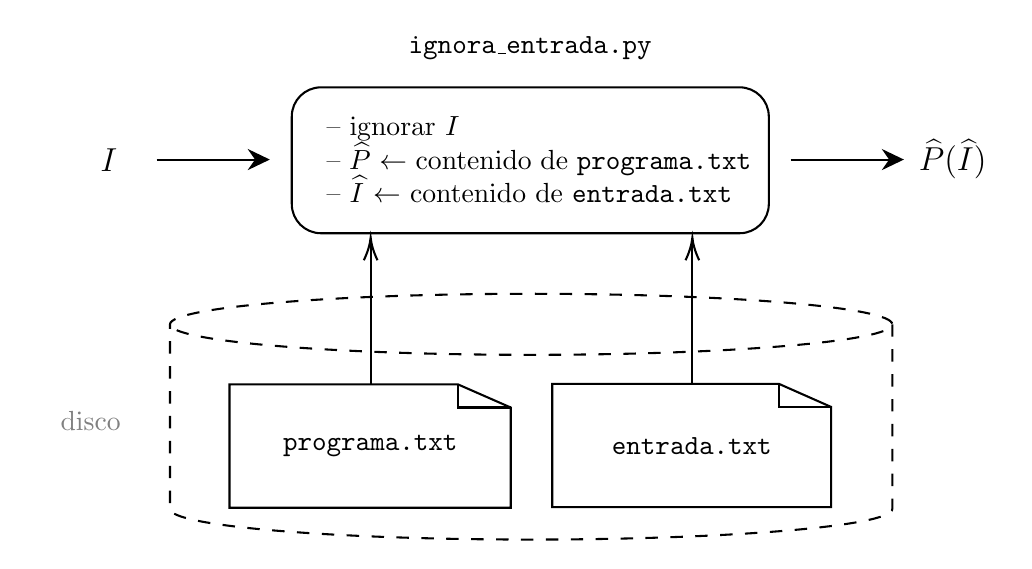
\begin{tikzpicture}[x=0.75pt,y=0.75pt,yscale=-1,xscale=1]
%uncomment if require: \path (0,446); %set diagram left start at 0, and has height of 446

%Rounded Rect [id:dp921706915568465] 
\draw   (220,155.73) .. controls (220,147.96) and (226.3,141.67) .. (234.06,141.67) -- (435.77,141.67) .. controls (443.54,141.67) and (449.83,147.96) .. (449.83,155.73) -- (449.83,197.91) .. controls (449.83,205.67) and (443.54,211.97) .. (435.77,211.97) -- (234.06,211.97) .. controls (226.3,211.97) and (220,205.67) .. (220,197.91) -- cycle ;
%Straight Lines [id:da5398342064124813] 
\draw    (154.83,176.47) -- (206.42,176.47) ;
\draw [shift={(209.42,176.47)}, rotate = 180] [fill={rgb, 255:red, 0; green, 0; blue, 0 }  ][line width=0.08]  [draw opacity=0] (10.72,-5.15) -- (0,0) -- (10.72,5.15) -- (7.12,0) -- cycle    ;
%Straight Lines [id:da5368997583766439] 
\draw    (460.33,176.47) -- (511.92,176.47) ;
\draw [shift={(514.92,176.47)}, rotate = 180] [fill={rgb, 255:red, 0; green, 0; blue, 0 }  ][line width=0.08]  [draw opacity=0] (10.72,-5.15) -- (0,0) -- (10.72,5.15) -- (7.12,0) -- cycle    ;
%Shape: Can [id:dp9670010852127255] 
\draw  [dash pattern={on 4.5pt off 4.5pt}] (509.33,255.84) -- (509.33,344.84) .. controls (509.33,352.97) and (431.43,359.55) .. (335.33,359.55) .. controls (239.24,359.55) and (161.33,352.97) .. (161.33,344.84) -- (161.33,255.84) .. controls (161.33,247.72) and (239.24,241.14) .. (335.33,241.14) .. controls (431.43,241.14) and (509.33,247.72) .. (509.33,255.84) .. controls (509.33,263.97) and (431.43,270.55) .. (335.33,270.55) .. controls (239.24,270.55) and (161.33,263.97) .. (161.33,255.84) ;
%Flowchart: Card [id:dp6407463317240687] 
\draw   (325.5,344.23) -- (325.5,295.94) -- (300.09,284.8) -- (190,284.8) -- (190,344.23) -- cycle ;
%Shape: Right Angle [id:dp1755547838848328] 
\draw   (325.5,295.94) -- (300.09,295.94) -- (300.09,284.8) ;
%Flowchart: Card [id:dp30404345921676557] 
\draw   (479.86,343.94) -- (479.86,295.66) -- (454.67,284.52) -- (345.5,284.52) -- (345.5,343.94) -- cycle ;
%Shape: Right Angle [id:dp6494941799046019] 
\draw   (479.86,295.66) -- (454.67,295.66) -- (454.67,284.52) ;
%Straight Lines [id:da5658612144537993] 
\draw    (258,284.55) -- (258,216.05) ;
\draw [shift={(258,214.05)}, rotate = 90] [color={rgb, 255:red, 0; green, 0; blue, 0 }  ][line width=0.75]    (10.93,-3.29) .. controls (6.95,-1.4) and (3.31,-0.3) .. (0,0) .. controls (3.31,0.3) and (6.95,1.4) .. (10.93,3.29)   ;
%Straight Lines [id:da4015405990035841] 
\draw    (413,284.55) -- (413,216.05) ;
\draw [shift={(413,214.05)}, rotate = 90] [color={rgb, 255:red, 0; green, 0; blue, 0 }  ][line width=0.75]    (10.93,-3.29) .. controls (6.95,-1.4) and (3.31,-0.3) .. (0,0) .. controls (3.31,0.3) and (6.95,1.4) .. (10.93,3.29)   ;

% Text Node
\draw (339.02,176.47) node  [color={rgb, 255:red, 0; green, 0; blue, 0 }  ,opacity=1 ] [align=left] {\begin{minipage}[lt]{153.43pt}\setlength\topsep{0pt}
\mbox{--} ignorar $I$\\\mbox{--} $\widehat{P}$ $\leftarrow$ contenido de \texttt{programa.txt}\\\mbox{--} $\widehat{I}$ $\leftarrow$ contenido de \texttt{entrada.txt}
\end{minipage}};
% Text Node
\draw (334.85,122.93) node  [color={rgb, 255:red, 0; green, 0; blue, 0 }  ,opacity=1 ] [align=left] {\begin{minipage}[lt]{155.92pt}\setlength\topsep{0pt}
\begin{center}
\texttt{ignora\_entrada.py}
\end{center}

\end{minipage}};
% Text Node
\draw (131.92,176.76) node  [font=\large,color={rgb, 255:red, 0; green, 0; blue, 0 }  ,opacity=1 ] [align=left] {\begin{minipage}[lt]{30.6pt}\setlength\topsep{0pt}
\begin{center}
$I$
\end{center}

\end{minipage}};
% Text Node
\draw (538.42,176.26) node  [font=\large,color={rgb, 255:red, 0; green, 0; blue, 0 }  ,opacity=1 ] [align=left] {\begin{minipage}[lt]{30.6pt}\setlength\topsep{0pt}
\begin{center}
$\widehat{P}(\widehat{I})$
\end{center}

\end{minipage}};
% Text Node
\draw (123.1,302.27) node  [color={rgb, 255:red, 128; green, 128; blue, 128 }  ,opacity=1 ] [align=left] {\begin{minipage}[lt]{38.85pt}\setlength\topsep{0pt}
\begin{center}
disco
\end{center}

\end{minipage}};
% Text Node
\draw (257.81,314.55) node  [color={rgb, 255:red, 0; green, 0; blue, 0 }  ,opacity=1 ] [align=left] {\begin{minipage}[lt]{91.6pt}\setlength\topsep{0pt}
\begin{center}
\texttt{programa.txt}
\end{center}

\end{minipage}};
% Text Node
\draw (412.74,314.27) node  [color={rgb, 255:red, 0; green, 0; blue, 0 }  ,opacity=1 ] [align=left] {\begin{minipage}[lt]{90.83pt}\setlength\topsep{0pt}
\begin{center}
\texttt{entrada.txt}
\end{center}

\end{minipage}};


\end{tikzpicture}
\caption{Esquema del programa \texttt{ignora\_entrada.py}}
\label{fig:ignora-entrada}
\end{figure}
% ====================

Para ello, usamos el \cref{lst:ignora-entrada}. Este programa, en lugar de ejecutar la entrada \linebreak\texttt{entrada\_ignorada}, ejecuta la máquina universal sobre un programa y una entrada almacenada en disco. Concretamente, usa como programa el almacenado en \texttt{disco/programa.txt}, y como entrada la almacenada en \texttt{disco/entrada.txt}.

Una vez conocemos el funcionamiento de \texttt{ignora\_entrada.py}, es sencillo encontrar una reducción de \textsc{Parada} a \textsc{ParadaEnVacío}.

\begin{proposicion}\label{prop:parada-en-vacio-no-decidible}
El problema \textsc{ParadaEnVacío} es no decidible.
\end{proposicion}
\begin{proof}
Basta hacer la reducción $\textsc{Parada}\leq_T\textsc{ParadaEnVacío}$ mediante el \cref{lst:parada-a-parada-en-vacio}. En efecto, vemos que tal programa resuelve \textsc{Parada}, asumiendo la existencia de un programa \texttt{parada\_en\_vacio.py} que resuelve \textsc{ParadaEnVacío}. Dado un programa \texttt{programa} y una entrada \texttt{entrada}, \texttt{parada\_a\_parada\_en\_vacio} almacenará los valores de las variables en \texttt{disco/programa.txt} y \texttt{disco/entrada.txt}, respectivamente, en las \cref{line:parada-a-parada-en-vacio-disco-programa,,line:parada-a-parada-en-vacio-disco-entrada}. A continuación, en la \cref{line:parada-a-parada-en-vacio-return} se devuelve si el programa \texttt{ignora\_entrada.py} para o no, lo que equivale a decir, por la forma en la que está escrito tal programa, si \texttt{programa} para con entrada \texttt{entrada}, resolviendo \textsc{Parada}.

El resultado se sigue de las \cref{prop:parada-no-decidible,,prop:decidible-reduccion}.
\end{proof}

\begin{lstlisting}[language=Python, caption=\lstinline{parada_a_parada_en_vacio.py},label={lst:parada-a-parada-en-vacio}]
import utilidades
from parada_en_vacio import parada_en_vacio # oráculo

def parada_a_parada_en_vacio(programa, entrada):
    utilidades.escribir('disco/programa.txt', programa)|\label{line:parada-a-parada-en-vacio-disco-programa}|
    utilidades.escribir('disco/entrada.txt', entrada)|\label{line:parada-a-parada-en-vacio-disco-entrada}|

    return parada_en_vacio(utilidades.leer('ignora_entrada.py'))|\label{line:parada-a-parada-en-vacio-return}|
\end{lstlisting}

Para concluir, introducimos un último problema: \textsc{AdivinaConsistente}. \cite{Aaronson2017}

\vspace{8pt}
% ====================
\begin{problema}
\begin{framed}
$$\text{\textsc{AdivinaConsistente}}$$

\begin{itemize}
    \item \textbf{Entrada:} un programa $P$.
    \item \textbf{Solución:} $\palabra{sí}$ si $P$ devuelve \palabra{sí} con entrada vacía (acepta), \palabra{no} en caso contrario (rechaza o cicla).
\end{itemize}
\end{framed}
\caption{\textsc{AdivinaConsistente}}
\label{prob:adivina-consistente}
\end{problema}
% ====================

La intuición nos indica que este problema, como los anteriores, tampoco es decidible. Lo probamos en la siguiente proposición.

\begin{proposicion}\label{prop:adivina-consistente-no-decidible}
\textsc{AdivinaConsistente} es no decidible.
\end{proposicion}
\begin{proof}
Asumiremos que \textsc{AdivinaConsistente} es decidible, entonces existe un programa \texttt{adivina\_consistente.py} que lo decide. En tal caso, podemos modificar \linebreak\texttt{adivina\_consistente.py} para crear un nuevo programa \texttt{modifica\_adivina\_consistente.py} (\cref{lst:modifica-adivina-consistente}), al que llamaremos $P$, que, dada una entrada \texttt{programa}, almacena en la variable \texttt{salida} (\cref{line:modifica-adivina-consistente-salida}):
\begin{itemize}
    \item \palabra{no} en caso de que \texttt{programa(programa) == \palabra{sí}}.
    \item \palabra{sí} en caso de que \texttt{programa(programa) == \palabra{no}}.
    \item \palabra{sí} en caso de que \texttt{programa(programa)} cicle (no pare).
\end{itemize}

Ahora, pensemos qué ocurre al ejecutar el programa sobre sí mismo, es decir, si pasamos el propio programa como entrada. Observemos antes que $P$ nunca ciclará, de acuerdo a la definición de \textsc{AdivinaConsistente}. Hay tres posibilidades:
\begin{itemize}
    \item Si $P(P)=\palabra{no}$, la única forma de que esto ocurra es si se verifica la condición de la \cref{line:modifica-adivina-consistente-return-no}, lo cual solo ocurre si $P(P)=\palabra{sí}$. Por tanto, esta posibilidad se descarta.
    \item Si $P(P)=\palabra{sí}$, la única forma de que esto pase es si se verifica la condición de la \cref{line:modifica-adivina-consistente-return-si}, lo cual solo ocurre si $P(P)=\palabra{no}$ o $P$ cicla, pero como $P$ nunca cicla, entonces deberá ser $P(P)=\palabra{no}$. También descartamos esta posibilidad.
    \item La única posibilidad es que $P(P)$ cicle, pero como hemos visto, esto no es posible.\vspace*{-0.8cm}
\end{itemize}
\end{proof}

\vspace{8pt}
\begin{lstlisting}[language=Python, caption=\lstinline{modifica_adivina_consistente.py},label={lst:modifica-adivina-consistente}]
import utilidades
from adivina_consistente import adivina_consistente # NO es un oráculo
from ignora_entrada import ignora_entrada

def modifica_adivina_consistente(programa):
    utilidades.escribir('disco/programa.txt', programa)
    utilidades.escribir('disco/entrada.txt', programa)

    salida = adivina_consistente(utilidades.leer('ignora_entrada.py'))|\label{line:modifica-adivina-consistente-salida}|

    if salida == 'sí':|\label{line:modifica-adivina-consistente-return-no}|
        return 'no'
    elif salida == 'no':|\label{line:modifica-adivina-consistente-return-si}|
        return 'sí'
\end{lstlisting}
% ====================

Los problemas \textsc{ParadaEnVacío} y \textsc{AdivinaConsistente} serán centrales en la demostración de dos variantes del resultado principal de este trabajo, en el \cref{ch:teorema-incompletitud}. A modo de resumen, se proporciona la \cref{tab:problemas} con todos los problemas presentados en este capítulo.

\pagebreak
\vspace*{3.5cm}
\begin{tabla}
\begin{table}[H]
\centering
\begin{tabular}{@{}llll@{}}
\cmidrule[0.7pt]{2-4}
 & Entrada & Salida & Decidible$\;\;$ \\ \midrule
\textsc{MásAQueB} & $u\in\{\palabra{a}, \palabra{b}\}^*$ & -- \palabra{sí}, si $\#(u,a)>\#(u,b)$ & sí \\
\small{(\cref{prob:mas-a-que-b})} && -- \palabra{no}, en caso contrario & \small{(\Cref{prop:masaqueb-decidible})}\\[4pt]
\textsc{Sí} & cualquiera & -- \palabra{sí} & sí \\
\small{(\cref{prob:si})} && & \small{(\Cpageref{lab:si-decidible})}\\[4pt]
\textsc{Universal} & $P$, $I$ & -- \palabra{sí}, si $P(I)=\palabra{sí}$ & no \\
\small{(\cref{prob:universal})} & & -- \palabra{no}, en caso contrario & \small{(\Cref{prop:universal-no-decidible})} \\[4pt]
\textsc{Diagonal} & $P$ & -- \palabra{sí}, si $P(P)=\palabra{sí}$ & no \\
\small{(\cref{prob:diagonal})} && -- \palabra{no}, en caso contrario& \small{(\Cpageref{lab:diagonal-no-decidible})}\\[4pt]
\textsc{C-Diagonal} & $P$ & -- \palabra{no}, si $P(P)=\palabra{sí}$ & no \\
\small{(\cref{prob:c-diagonal})} && -- \palabra{sí}, en caso contrario& \small{(\Cref{prop:c-diagonal-no-decidible})}\\[4pt]
\textsc{Parada} & $P$, $I$ & -- \palabra{sí}, si $P$ para con entrada $I$ & no \\
\small{(\cref{prob:parada})} & & -- \palabra{no}, en caso contrario& \small{(\Cref{prop:parada-no-decidible})}\\[4pt]
\textsc{ParadaEnVacío} & $P$ & -- \palabra{sí}, si $P$ para con entrada \palabra{} & no \\
\small{(\cref{prob:parada-en-vacio})} & & -- \palabra{no}, en caso contrario& \small{(\Cref{prop:parada-en-vacio-no-decidible})}\\[4pt]
\textsc{AdivinaConsistente} & $P$ & -- \palabra{sí}, si $P(\palabra{})$ para y $P(\palabra{})=\palabra{sí}$ & no \\
\small{(\cref{prob:adivina-consistente})} &  & -- \palabra{no}, si $P(\palabra{})$ para y $P(\palabra{})\neq\palabra{sí}$ & \small{(\Cref{prop:adivina-consistente-no-decidible})}\\
&& -- \palabra{no}, si $P(\palabra{})$ cicla\\\bottomrule
\end{tabular}
\end{table}
\vspace{-8pt}
\caption{Resumen de los problemas presentados en este capítulo}
\label{tab:problemas}
\end{tabla}
% ====================
\endinput

